%% abtex2-modelo-trabalho-academico.tex, v-1.9.2 laurocesar
%% Copyright 2012-2014 by abnTeX2 group at http://abntex2.googlecode.com/ 
%%
%% This work may be distributed and/or modified under the
%% conditions of the LaTeX Project Public License, either version 1.3
%% of this license or (at your option) any later version.
%% The latest version of this license is in
%%   http://www.latex-project.org/lppl.txt
%% and version 1.3 or later is part of all distributions of LaTeX
%% version 2005/12/01 or later.
%%
%% This work has the LPPL maintenance status `maintained'.
%% 
%% The Current Maintainer of this work is the abnTeX2 team, led
%% by Lauro César Araujo. Further information are available on 
%% http://abntex2.googlecode.com/
%%
%% This work consists of the files abntex2-modelo-trabalho-academico.tex,
%% abntex2-modelo-include-comandos and abntex2-modelo-references.bib
%%

% ------------------------------------------------------------------------
% ------------------------------------------------------------------------
% abnTeX2: Modelo de Trabalho Academico (tese de doutorado, dissertacao de
% mestrado e trabalhos monograficos em geral) em conformidade com 
% ABNT NBR 14724:2011: Informacao e documentacao - Trabalhos academicos -
% Apresentacao
% ------------------------------------------------------------------------
% ------------------------------------------------------------------------

%-------------------------------------------------------------------------
% Modelo adaptado especificamente para o contexto do PPgSI-EACH-USP por 
% Marcelo Fantinato, com auxílio dos Professores Norton T. Roman, Helton
% H. Bíscaro e Sarajane M. Peres, em 2015, com muitos agradecimentos aos 
% criadores da classe e do modelo base.
%
% 20/06/2017: inclusão de "lista de quadros" com base no especificado em:
% https://github.com/abntex/abntex2/wiki/HowToCriarNovoAmbienteListing,
% de autoria de "Eduardo de Santana Medeiros Alexandre".
%
%-------------------------------------------------------------------------

\documentclass[
	% -- opções da classe memoir --
	12pt,				% tamanho da fonte
	% openright,			% capítulos começam em pág ímpar (insere página vazia caso preciso)
	oneside,			% para impressão apenas no anverso (apenas frente). Oposto a twoside
	a4paper,			% tamanho do papel. 
	% -- opções da classe abntex2 --
	%chapter=TITLE,		% títulos de capítulos convertidos em letras maiúsculas
	%section=TITLE,		% títulos de seções convertidos em letras maiúsculas
	%subsection=TITLE,	% títulos de subseções convertidos em letras maiúsculas
	%subsubsection=TITLE,% títulos de subsubseções convertidos em letras maiúsculas
	% -- opções do pacote babel --
	english,			% idioma adicional para hifenização
	%french,				% idioma adicional para hifenização
	%spanish,			% idioma adicional para hifenização
	brazil				% o último idioma é o principal do documento
	]{abntex2ppgsi}

% ---
% Pacotes básicos 
% ---
% \usepackage{lmodern}			% Usa a fonte Latin Modern			
% \usepackage[T1]{fontenc}		% Selecao de codigos de fonte.
\usepackage[utf8]{inputenc}		% Codificacao do documento (conversão automática dos acentos)
\usepackage{lastpage}			% Usado pela Ficha catalográfica
\usepackage{indentfirst}		% Indenta o primeiro parágrafo de cada seção.
\usepackage{color}				% Controle das cores
\usepackage{graphicx}			% Inclusão de gráficos
\usepackage{microtype} 			% para melhorias de justificação
\usepackage{pdfpages}     %para incluir pdf
\usepackage{algorithm}			%para ilustrações do tipo algoritmo
\usepackage{mdwlist}			%para itens com espaço padrão da abnt
\usepackage[noend]{algpseudocode}			%para ilustrações do tipo algoritmo
\usepackage{chemformula} % para escrever CO2 corretamente
\usepackage{longtable} % para tabelas longas
\usepackage{pgfgantt}
		
% ---
% Pacotes adicionais, usados apenas no âmbito do Modelo Canônico do abnteX2
% ---
\usepackage{lipsum}				% para geração de dummy text
% ---

% ---
% Pacotes de citações
% ---
\usepackage{hyperref}
\usepackage[brazilian,hyperpageref]{backref}	 % Paginas com as citações na bibl
\usepackage[alf,abnt-etal-list=0,abnt-etal-text=it]{abntex2cite}	% Citações padrão ABNT

% --- 
% CONFIGURAÇÕES DE PACOTES
% --- 

% ---
% Configurações do pacote backref
% Usado sem a opção hyperpageref de backref
\renewcommand{\backrefpagesname}{Citado na(s) página(s):~}
% Texto padrão antes do número das páginas
\renewcommand{\backref}{}
% Define os textos da citação
\renewcommand*{\backrefalt}[4]{
	\ifcase #1 %
		Nenhuma citação no texto.%
	\or
		Citado na página #2.%
	\else
		Citado #1 vezes nas páginas #2.%
	\fi}%
% ---

% ---
% Informações de dados para CAPA e FOLHA DE ROSTO
% ---
\instituicao{
	UNIVERSIDADE DE SÃO PAULO
	\par
	ESCOLA DE ARTES, CIÊNCIAS E HUMANIDADES
	\par
	PROGRAMA DE PÓS-GRADUAÇÃO EM SISTEMAS DE INFORMAÇÃO}

%-------------------------------------------------------------------------
% Comentário adicional do PPgSI - Informações sobre o ``título'':
%
% Em maiúscula apenas a primeira letra da sentença (do título), exceto 
% nomes próprios, geográficos, institucionais ou Programas ou Projetos ou 
% siglas, os quais podem ter letras em maiúscula também.
%
% O subtítulo do trabalho é opcional.
% Sem ponto final.
%
% Atenção: o título da Dissertação/Tese na versão corrigida não pode mudar. 
% Ele deve ser idêntico ao da versão original.
%
%-------------------------------------------------------------------------
\titulo{Estratégias de migração de máquinas virtuais para a redução da pegada de carbono na computação em nuvem verde}
\autor{\uppercase{Guilherme Fernandes Moraes da Silva}}
\local{São Paulo}

%-------------------------------------------------------------------------
% Comentário adicional do PPgSI - Informações sobre a ``data'':
%
% Colocar o ano do depósito (ou seja, o ano da entrega) da respectiva 
% versão, seja ela a versão original (para a defesa) seja ela a versão 
% corrigida (depois da aprovação na defesa). 
%
% Atenção: Se a versão original for depositada no final do ano e a versão 
% corrigida for entregue no ano seguinte, o ano precisa ser atualizado no 
% caso da versão corrigida. 
% Cuidado, pois o ano da ``capa externa'' também precisa ser atualizado 
% nesse caso.
%
% Não incluir o dia, nem o mês.
% Sem ponto final.
%-------------------------------------------------------------------------
\data{2024}
\orientador{Prof. Dr. Daniel de Angelis Cordeiro}
\tipotrabalho{Dissertação (Mestrado) / Tese (Doutorado)}

\preambulo{
Projeto de pesquisa para exame de qualificação apresentado à Escola de Artes, Ciências e Humanidades da Universidade de São Paulo como parte dos requisitos para obtenção do título de Mestre em Ciências pelo Programa de Pós-graduação em Sistemas de Informação.
\newline \newline Área de concentração: Metodologia e Técnicas da Computação
}

% ---
% Configurações de aparência do PDF final

% alterando o aspecto da cor azul
\definecolor{blue}{RGB}{41,5,195}

% informações do PDF
\makeatletter
\hypersetup{
     	%pagebackref=true,
		pdftitle={\@title}, 
		pdfauthor={\@author},
    	pdfsubject={\imprimirpreambulo},
	    pdfcreator={laTeX com abnTeX2 adaptado para o PPgSI-EACH-USP},
		pdfkeywords={abnt}{latex}{abntex}{abntex2ppgsi}{qualificação de mestrado}{dissertação de mestrado}{qualificação de doutorado}{tese de doutorado}{ppgsi}, 
		colorlinks=true,       		% false: boxed links; true: colored links
    	linkcolor=blue,          	% color of internal links
    	citecolor=blue,        		% color of links to bibliography
    	filecolor=magenta,      		% color of file links
		urlcolor=blue,
		bookmarksdepth=4
}
\makeatother
% --- 

% --- 
% Espaçamentos entre linhas e parágrafos 
% --- 

% O tamanho do parágrafo é dado por:
\setlength{\parindent}{1.25cm}

% Controle do espaçamento entre um parágrafo e outro:
\setlength{\parskip}{0cm}  % tente também \onelineskip
\renewcommand{\baselinestretch}{1.5}

% ---
% compila o indice
% ---
\makeindex
% ---

	% Controlar linhas orfas e viuvas
  \clubpenalty10000
  \widowpenalty10000
  \displaywidowpenalty10000

% ----
% Início do documento
% ----
\begin{document}

% Retira espaço extra obsoleto entre as frases.
\frenchspacing 

% ----------------------------------------------------------
% ELEMENTOS PRÉ-TEXTUAIS
% ----------------------------------------------------------
% \pretextual

% ---
% Capa
% ---
%-------------------------------------------------------------------------
% Comentário adicional do PPgSI - Informações sobre a ``capa'':
%
% Esta é a ``capa'' principal/oficial do trabalho, a ser impressa apenas 
% para os casos de encadernação simples (ou seja, em ``espiral'' com 
% plástico na frente).
% 
% Não imprimir esta ``capa'' quando houver ``capa dura'' ou ``capa brochura'' 
% em que estas mesmas informações já estão presentes nela.
%
%-------------------------------------------------------------------------
\imprimircapa
% ---

% ---
% Folha de rosto
% (o * indica que haverá a ficha bibliográfica)
% ---
\imprimirfolhaderosto*
% ---

% ---
% ---
% inserir lista de figuras
% ---
\pdfbookmark[0]{\listfigurename}{lof}
\listoffigures*
\cleardoublepage
% ---

% ---
% inserir lista de abreviaturas e siglas
% ---
%-------------------------------------------------------------------------
% Comentário adicional do PPgSI - Informações sobre ``Lista de abreviaturas 
% e siglas'': 
%
% Opcional.
% Uma vez que se deseja usar, é necessário manter padrão e consistência no
% trabalho inteiro.
% Se usar: inserir em ordem alfabética.
%
%-------------------------------------------------------------------------
\begin{siglas}
  \item[CRC] \textit{Carbon-responsive computing}
  \item[DC] \textit{Data center}
  \item[IaaS] \textit{Infrastructure as a Service}
  \item[PaaS] \textit{Platform as a Service}
  \item[SaaS] \textit{Software as a Service}
  \item[TI] Tecnologia da informação
  \item[VM] Máquina virtual
  \item[VMM] Monitor de máquina virtual
\end{siglas}
% ---


% ---
% inserir lista de símbolos
% ---
%-------------------------------------------------------------------------
% Comentário adicional do PPgSI - Informações sobre ``Lista de símbolos'': 
%
% Opcional.
% Uma vez que se deseja usar, é necessário manter padrão e consistência no
% trabalho inteiro.
% Se usar: inserir na ordem em que aparece no texto.
% 
%-------------------------------------------------------------------------
\begin{simbolos}
	\item[$ \alpha $] Letra grega minúscula Alfa
	\item[$ \beta $] Letra grega minúscula Beta
	\item[$ \gamma $] Letra grega minúscula Gama
  \end{simbolos}
  % ---

% ---
% inserir o sumario
% ---
\pdfbookmark[0]{\contentsname}{toc}
\tableofcontents*
\cleardoublepage
% ---



% ----------------------------------------------------------
% ELEMENTOS TEXTUAIS
% ----------------------------------------------------------
\textual



%-------------------------------------------------------------------------
% Comentário adicional do PPgSI - Informações sobre ``títulos de seções''
% 
% Para todos os títulos (seções, subseções, tabelas, ilustrações, etc.):
%
% Em maiúscula apenas a primeira letra da sentença (do título), exceto 
% nomes próprios, geográficos, institucionais ou Programas ou Projetos ou
% siglas, os quais podem ter letras em maiúscula também.
%
%-------------------------------------------------------------------------
\chapter{Introdução}
A computação em nuvem desempenha um papel central na sociedade moderna, sustentando desde atividades cotidianas até operações críticas em grandes corporações e governos. À medida que a adoção de serviços de nuvem cresce, os \textit{data centers} (DCs) tornaram-se essenciais para essa infraestrutura. No entanto, esse avanço traz desafios significativos, especialmente relacionados ao consumo energético e às emissões de \ch{CO2}. A sustentabilidade desse crescimento depende de inovações que conciliem eficiência operacional e redução de impactos ambientais.

Um dos problemas críticos enfrentados é o alto consumo energético de DCs, intensificado pela dependência de fontes de energia de alta intensidade de carbono em diversas regiões. Para abordar esses desafios, estratégias como a migração de máquinas virtuais (VMs) têm ganhado destaque, oferecendo uma forma de otimizar recursos e priorizar o uso de fontes de energia renováveis.

Este trabalho propõe investigar como algoritmos para a migração de VMs podem ser desenvolvidos e otimizados para reduzir as emissões de carbono, mitigar problemas como \textit{downtime} de aplicações e congestionamento de rede, e maximizar o uso de energia limpa em \textit{data centers} geodistribuídos. Para isso, serão desenvolvidas e realizadas simulações computacionais utilizando métricas padronizadas para avaliar a eficiência de diferentes abordagens.

\section{Contextualização}
A computação em nuvem tornou-se uma infraestrutura essencial para atender às demandas crescentes da sociedade moderna. Com o aumento exponencial de dados e serviços, os \textit{data centers} (DCs) desempenham um papel crucial nesse ecossistema. Entre 2010 e 2018, as demandas de DCs cresceram substancialmente, com aumentos significativos no tráfego IP, armazenamento e carga de trabalho, conforme \citeonline{doi:10.1126/science.aba3758}. Apesar dos avanços na eficiência energética, projeções futuras indicam cenários preocupantes de aumento no consumo energético, especialmente em regiões onde fontes de energia de alta intensidade de carbono predominam \cite{KOOT2021116798}.

Paralelamente, eventos globais como a pandemia de COVID-19 demonstraram a vulnerabilidade do setor a mudanças repentinas na demanda, intensificando a pressão sobre as infraestruturas de DCs, de acordo com \citeonline{10.1145/3419394.3423658}. Essa pressão evidencia a necessidade de soluções tecnológicas que integrem eficiência operacional e sustentabilidade ambiental.

Nesse contexto, a migração de VMs surge como uma solução promissora. Ela permite a alocação dinâmica de cargas de trabalho em DCs que utilizam energia limpa, reduzindo as emissões de carbono associadas. Contudo, essa abordagem apresenta desafios técnicos, como \textit{downtime} de aplicações, congestionamento de rede e eficiência operacional, que devem ser cuidadosamente equilibrados para maximizar seus benefícios.

\section{Justificativa}
A crescente demanda por serviços de computação em nuvem tem levado a uma expansão significativa na utilização de DCs, acompanhada de impactos ambientais consideráveis. Apesar dos avanços na eficiência energética, como destacado por \citeonline{doi:10.1126/science.aba3758}, o crescimento contínuo das cargas de trabalho e do tráfego digital impede uma redução efetiva do consumo energético global. Isso se agrava devido à dependência de fontes de energia de alta intensidade de carbono em muitas regiões, como a Virgínia, que processa grande parte do tráfego de internet dos EUA e utiliza predominantemente fontes fósseis \cite{clicking_clean_virginia}.

Essa realidade evidencia lacunas importantes no setor. Primeiro, enquanto estratégias para melhorar a eficiência energética são bem documentadas, há pouca padronização na avaliação de técnicas voltadas à redução de emissões de carbono em DCs. Isso dificulta a comparação objetiva entre algoritmos e impede a replicabilidade de experimentos existentes. Segundo, soluções como a migração de VMs apresentam potencial para minimizar emissões de \ch{CO2} ao alocar cargas de trabalho para locais que utilizam energia de baixa intensidade de carbono. No entanto, a literatura atual é limitada em estudos que combinem algoritmos ou avaliem estratégias híbridas de forma sistemática, deixando uma lacuna relevante a ser explorada.

Além disso, questões práticas, como \textit{downtime} das aplicações e congestionamento da rede, são frequentemente tratadas de forma isolada, sem considerar o impacto combinado com o uso de energia limpa. Isso revela a necessidade de soluções que integrem múltiplos critérios, equilibrando sustentabilidade ambiental e eficiência operacional.

A relevância desse estudo é reforçada pelo alinhamento com objetivos globais de sustentabilidade, como os acordos internacionais para reduzir emissões de gases de efeito estufa e metas corporativas de neutralidade de carbono, como reforça \citeonline{nations_emissions_2024}. Empresas de tecnologia líderes, como Google e Microsoft, já sinalizaram o compromisso com práticas sustentáveis, mas a implementação prática dessas metas depende de abordagens técnicas robustas \cite{Google_Microsoft_Climate_Change}.

Portanto, o desenvolvimento de algoritmos eficientes para a migração de VMs em DCs geodistribuídos representa uma contribuição significativa tanto para a pesquisa acadêmica quanto para a prática industrial. Este trabalho busca preencher essas lacunas, propondo soluções que atendam simultaneamente às necessidades ambientais, econômicas e operacionais da computação em nuvem.

\section{Problema de pesquisa}
Como otimizar a migração de VMs em DCs geodistribuídos para minimizar as emissões de \ch{CO2}, reduzir o \textit{downtime} das aplicações, evitar o congestionamento da rede e maximizar o uso de fontes de energia de baixa intensidade de carbono, considerando as lacunas existentes na padronização de experimentos e na integração de diferentes algoritmos e técnicas?

\section{Questões de pesquisa}
\textbf{Q1:} Quais algoritmos ou técnicas de migração existentes de VMs em DCs geodistribuídos são mais eficientes para minimizar as emissões de \ch{CO2}?

\textbf{Q2:} Qual é o ganho quantitativo obtido ao mesclar diferentes algoritmos ou técnicas de migração em termos de redução de emissões de \ch{CO2} e outros critérios relevantes, especialmente em cenários com fontes de energia renováveis?

\section{Objetivos}
Nesta seção, são definidos os objetivos que guiarão o desenvolvimento e a condução deste trabalho de pesquisa. Primeiramente, o objetivo geral (\ref{subsection:objetivo-geral}) é apresentado, abrangendo a meta principal a ser alcançada com o estudo. Em seguida, os objetivos específicos (\ref{subsection:objetivos-especificos}) detalham as metas secundárias que, de forma integrada, contribuem para o atingimento do objetivo geral, fornecendo uma estrutura clara para responder às questões de pesquisa propostas.

\subsection{Objetivo geral}\label{subsection:objetivo-geral}
Desenvolver e validar um algoritmo para a migração de VMs em DCs geodistribuídos capaz de minimizar as emissões de \ch{CO2}, reduzir o \textit{downtime} das aplicações, evitar congestionamento de rede e maximizar o uso de fontes de energia de baixa intensidade de carbono.

\subsection{Objetivos específicos}\label{subsection:objetivos-especificos}
\begin{itemize}
	\item Identificar e analisar os algoritmos e técnicas existentes na literatura, avaliando sua eficiência em minimizar emissões de \ch{CO2} e outros critérios relevantes, como \textit{downtime} e congestionamento de rede, em cenários de DCs geodistribuídos.
	\item Desenvolver um algoritmo integrado que otimize simultaneamente critérios ambientais, como a redução de emissões de \ch{CO2}, e critérios operacionais, como o tempo de indisponibilidade das aplicações e o congestionamento da rede.
\end{itemize}

\section{Método de pesquisa}
O método de pesquisa adotado nesta dissertação baseia-se em simulações computacionais para modelar, implementar e avaliar cenários de migração de máquinas virtuais (VMs) em \textit{data centers} geodistribuídos. As simulações serão desenvolvidas utilizando o \textit{framework} SimGrid por \citeonline{casanova:hal-01017319}, uma ferramenta amplamente validada pela comunidade científica e utilizada há mais de 20 anos para modelar experimentos de computação distribuída, como plataformas de nuvem. A escolha do SimGrid se justifica pela sua capacidade de modelar com precisão o consumo de energia na execução das tarefas, o processo de ligar e desligar servidores, o uso da rede durante a migração ao vivo, a topologia da rede e o congestionamento da rede. Outro ponto importante para sua escolha é que, apesar de ser possível realizar simulações em nível de pacotes para maior precisão, isso acarretaria um tempo de execução significativamente mais longo. O modelo de nível de fluxo TCP padrão do SimGrid, por outro lado, proporciona resultados precisos em cenários de computação distribuída em larga escala, como o que será utilizado neste trabalho, com milhares de servidores, e em um tempo razoável de execução \cite{velho:hal-00872476}.

Os cenários experimentais serão projetados para refletir ambientes realistas de DCs geodistribuídos, levando em consideração variações nos perfis de carga de trabalho, nas fontes de energia e na topologia da rede. Serão implementados algoritmos existentes para migração de VMs com foco na minimização de \ch{CO2}, \textit{downtime}, congestionamento de rede e otimização do uso de fontes de energia de baixa intensidade de carbono. A implementação buscará garantir a reprodutibilidade dos experimentos e a comparação direta entre as técnicas de migração.

Para considerar o impacto ambiental dos servidores, será utilizada a metodologia proposta por \citeonline{10.1145/3470496.3527408}, que apresenta uma abordagem detalhada para calcular a pegada de carbono dos componentes de \textit{hardware} dos servidores. Essa metodologia inclui o cálculo das emissões relacionadas à fabricação de circuitos integrados de RAM, armazenamento (HDs e SSDs) e CPU. Incorporar esse aspecto permitirá uma análise mais completa das emissões de \ch{CO2}, não apenas durante a operação dos DCs, mas também em seu ciclo de vida completo.

Os testes serão conduzidos utilizando métricas padronizadas para avaliar o desempenho dos algoritmos em relação aos objetivos propostos. Entre as métricas previstas estão: redução de emissão de \ch{CO2}, impacto no \textit{downtime} das aplicações, eficiência no uso da rede e aderência ao uso de energia limpa. A utilização do mesmo simulador e dos mesmos cenários experimentais permitirá a comparação direta entre os algoritmos, identificando suas vantagens e limitações.

Além disso, será investigada a viabilidade e a efetividade de combinar diferentes algoritmos ou técnicas para obter melhores resultados. Essa etapa envolve a análise de sinergias entre as abordagens, buscando estratégias híbridas que aproveitem as vantagens de cada método.

Os resultados obtidos serão analisados criticamente para identificar as condições em que os algoritmos ou combinações propostas apresentam melhor desempenho. A confiabilidade dos resultados será validada por meio de replicações e variações nos cenários experimentais. Por fim, as conclusões serão discutidas em relação às lacunas e limitações apontadas na literatura, destacando as contribuições desta pesquisa e possíveis extensões futuras.

\section{Cronograma proposto}
O diagrama abaixo apresenta o cronograma de atividades previstas para a realização desta pesquisa, distribuídas entre agosto de 2024 e maio de 2026. As etapas foram organizadas para garantir um desenvolvimento estruturado, permitindo a conclusão antecipada para lidar com possíveis imprevistos.

\begin{centering}
	\begin{ganttchart}[
	y unit title=0.5cm,
	y unit chart=0.8cm,
	expand chart=\textwidth,
	hgrid,vgrid,
	title height=1,
	bar/.style={fill=gray, rounded corners=3pt},
	group/.style={fill=black, rounded corners=3pt},
	bar height=.2,
	progress label text={},
	group left shift=0.05,
	bar left shift=0.05,
	group height=.3,
	group peaks width={0.0},
	inline]{1}{24}
 
   \gantttitle[]{\textbf{2024}}{6}
   \gantttitle[]{\textbf{2025}}{12}
   \gantttitle[]{\textbf{2026}}{6}

   \ganttnewline
   
   \gantttitle{\textbf{Q3}}{3}
   \gantttitle{\textbf{Q4}}{3}
   \gantttitle{\textbf{Q1}}{3}
   \gantttitle{\textbf{Q2}}{3}
   \gantttitle{\textbf{Q3}}{3}
   \gantttitle{\textbf{Q4}}{3}
   \gantttitle{\textbf{Q1}}{3}
   \gantttitle{\textbf{Q2}}{3}

   \ganttnewline

   \ganttgroup[inline=false]{Qualificação}{3}{10.5}\\ 
   \ganttbar[inline=false]{Fundamentação teórica}{1}{3}\\
   \ganttbar[inline=false]{Método de pesquisa}{3}{6}\\
   \ganttbar[inline=false]{Introdução}{4}{6}\\
   \ganttbar[inline=false]{Questões de pesquisa}{3}{5}\\
   \ganttbar[inline=false]{Problema de pesquisa}{3.5}{5.5}\\
   \ganttbar[inline=false]{Trabalhos correlatos}{5}{8}\\
   \ganttbar[inline=false]{Limitações e riscos}{4.5}{6.5}\\
   \ganttbar[inline=false]{Objetivo geral}{5}{7} \\
   \ganttbar[inline=false]{Objetivos específicos}{5}{7}

   \ganttnewline[ultra thick]

   \ganttgroup[inline=false]{Experimentos}{7}{17}\\
   \ganttbar[inline=false]{Estado da Arte}{5}{15}\\
   \ganttbar[inline=false]{Aperfeiçoamentos}{14}{18}

   \ganttnewline[ultra thick]
   
   \ganttgroup[inline=false]{Dissertação}{6}{23.5}\\
   \ganttbar[inline=false]{Comparativos}{7}{18}\\
   \ganttbar[inline=false]{Releituras}{7}{23}

   \ganttvrule[vrule offset=.5]{Qualificação}{11}
   \ganttvrule[vrule offset=.5]{Defesa da Dissertação}{24.5}
\end{ganttchart}
\end{centering}

Na fase inicial, entre agosto e dezembro de 2024, está planejado o desenvolvimento da fundamentação teórica, a análise de trabalhos correlatos, e a formulação das questões de pesquisa e do problema de pesquisa. Durante esse período, também serão definidos os métodos de pesquisa, os objetivos gerais e específicos, bem como a introdução e análise de riscos associados ao trabalho. Paralelamente, inicia-se a elaboração preliminar da dissertação, incorporando os capítulos já desenvolvidos, e as primeiras releituras críticas para garantir consistência.

A partir de janeiro de 2025, inicia-se a segunda fase, com a realização do levantamento do estado da arte até março, proporcionando uma visão abrangente e atualizada sobre os algoritmos e técnicas relacionadas à migração de VMs em DCs geodistribuídos. De janeiro a novembro, serão conduzidos os experimentos, nos quais as técnicas identificadas serão testadas e analisadas sob cenários variados. Paralelamente, os resultados desses experimentos serão utilizados para a escrita contínua da dissertação, que será progressivamente atualizada e revisada com base nos avanços obtidos. Entre julho e janeiro de 2026, serão implementados aperfeiçoamentos nos algoritmos propostos, alinhados aos objetivos de redução de emissões de \ch{CO2} e eficiência operacional.

A terceira fase, de dezembro de 2025 a maio de 2026, será dedicada à consolidação dos resultados comparativos, realizados ao longo do desenvolvimento, com a análise final ocorrendo entre janeiro e março de 2026. Nesse período, o foco estará na finalização e revisão da dissertação, garantindo a integração de todos os capítulos produzidos, bem como na realização de releituras detalhadas para assegurar a coesão do texto e o atendimento aos objetivos da pesquisa. O encerramento está planejado para maio de 2026, três meses antes do prazo final, reservando uma margem de segurança para eventuais ajustes e imprevistos.

\section{Limitações e riscos}
A pesquisa apresenta algumas limitações e riscos inerentes à natureza do problema e ao método adotado. Um dos principais aspectos é a dependência de simuladores para realizar os testes e comparações dos algoritmos de migração de VMs. Embora simuladores sejam amplamente utilizados na literatura por sua capacidade de modelar cenários complexos de DCs geodistribuídos, eles não capturam de forma completa todas as variáveis e incertezas de ambientes reais. Isso pode limitar a generalização dos resultados para infraestruturas físicas.

Além disso, a rápida evolução tecnológica no setor de computação em nuvem e o surgimento de novos paradigmas podem reduzir a relevância dos resultados obtidos caso novas práticas substituam as tecnologias abordadas.

Essas limitações e riscos serão mitigados, na medida do possível, por meio de uma seleção criteriosa de simuladores e uma análise crítica dos experimentos realizados. Contudo, reconhece-se que os resultados da pesquisa são direcionados a contextos modelados e devem ser avaliados sob essa perspectiva.


\section{Estrutura do documento}
Este trabalho está organizado nos seguintes capítulos. No Capítulo \ref{chapter:fundamentacao-teorica}, apresenta-se os conceitos fundamentais usados no restante deste trabalho ou necessários para o entendimento do mesmo. No Capítulo \ref{chapter:trabalhos-correlatos}, discute-se sobre os trabalhos relacionados que de algum modo se conectam a esta pesquisa, identificando avanços, lacunas e oportunidades. Adicionalmente, o Apêndice \ref{chapter:protocolo-revisao-estado-da-arte} e Apêndice \ref{chapter:resultados-conducao-revisao-estado-da-arte} incluem detalhes complementares, como o protocolo e os resultados da revisão do estado da arte.

\chapter{Fundamentação teórica}\label{chapter:fundamentacao-teorica}

Neste capítulo são apresentados conceitos fundamentais para o leitor entender os demais capítulos desta dissertação. Primeiro, os conceitos de máquinas virtuais e migração de máquinas virtuais são apresentados na Seção \ref{section:maquinas-virtuais}. Em seguida, a Seção \ref{section:computacao-nuvem} apresenta os conceitos de computação em nuvem e computação em nuvem verde, além de fornecer uma visão geral sobre esses temas atualmente. Por fim, a Seção \ref{section:escalonamento} introduz o conceito de escalonamento e como ele é utilizado no contexto de computação em nuvem.

\section{Máquinas Virtuais}\label{section:maquinas-virtuais}

Uma máquina virtual (VM) é um ambiente virtualizado criado pelo hipervisor, também conhecido como monitor de máquina virtual (VMM). O VMM gerencia os recursos físicos do sistema anfitrião (a máquina física) e provisiona múltiplos ambientes virtuais independentes, chamados de convidados. Sua função principal é garantir que essas VMs compartilhem os recursos físicos de forma eficiente, evitando, por exemplo, que a mesma região de memória seja alocada simultaneamente para mais de uma VM. Dessa forma, a VM atua como uma duplicata isolada e eficiente de uma máquina real, permitindo a execução de sistemas operacionais e aplicações de forma independente e segura \cite{10.1145/361011.361073}.

Entre a máquina física e as VMs, há uma camada de \textit{software} que possibilita a virtualização dos recursos. Essa camada, controlada pelo VMM, permite que as VMs superem as limitações de compatibilidade de \textit{hardware} e recursos, criando um ambiente mais flexível. Em sistemas tradicionais de virtualização, o VMM opera com os mais altos privilégios, enquanto as VMs funcionam com privilégios reduzidos. Isso garante que o hipervisor possa interceptar e controlar ações que, de outra forma, acessariam ou modificariam componentes críticos do \textit{hardware}, assegurando o isolamento entre as VMs e a estabilidade do sistema anfitrião. Com essa separação, torna-se possível executar diversos sistemas operacionais ou aplicações simultaneamente em uma única máquina física, o que maximiza o uso dos recursos e melhora a eficiência do ambiente computacional \cite{1430629}.

A implementação de tecnologias de virtualização também relaxa as restrições impostas pelo \textit{hardware}, e amplia a flexibilidade do sistema. A virtualização oferece um ambiente abstrato e isolado para a execução de aplicações, o que permite maior escalabilidade e facilita o gerenciamento de recursos. Além disso, existe um vasto conjunto de tecnologias e conceitos que tornam essa abstração possível, proporcionando uma infraestrutura mais adaptável às demandas dinâmicas da computação moderna \cite{10.5555/2531413}.

\subsection{Migração ao vivo de Máquinas Virtuais}\label{section:migracao-ao-vivo-maquinas-virtuais}

A migração ao vivo de máquinas virtuais é um processo útil para a administração de \textit{data centers} e \textit{clusters}, pois separa o \textit{hardware} do \textit{software}, o que facilita o gerenciamento de falhas, balanceamento de carga e manutenção. Ao transferir o sistema operacional e suas aplicações como uma unidade, esse processo permite mover o estado em memória de forma eficiente e consistente, garantindo a continuidade da execução sem interrupções. Uma das principais vantagens dessa abordagem é a possibilidade de desativar a máquina original após a conclusão da migração, o que é especialmente útil para realizar a manutenção do \textit{hardware}. Ao migrar a máquina virtual completa, o processo ocorre de forma transparente para os serviços em execução, eliminando a necessidade de gerenciar detalhes internos da VM. Isso permite, por exemplo, a migração de servidores de jogos \textit{online} sem desconectar os usuários, algo inviável em métodos que dependem da reinicialização no nível da aplicação ou do redirecionamento na camada de aplicação \cite{10.5555/1251203.1251223}.

\section{Computação em nuvem}\label{section:computacao-nuvem}

A computação em nuvem surgiu como uma solução para um dos maiores desafios da indústria tecnológica: a necessidade de que usuários e empresas adquirissem e mantivessem sua própria infraestrutura para disponibilizar serviços e aplicações. Com o crescimento exponencial da \textit{internet}, a tarefa de escalar essa infraestrutura para atender à demanda crescente tornou-se cada vez mais complexa e custosa. Conforme \citeonline{4738445}, a computação em nuvem pode ser definida como um paradigma de computação distribuída em larga escala, impulsionado pelas economias de escala, no qual um conjunto de recursos --- como computação, armazenamento, plataformas e serviços --- é abstraído, virtualizado, escalonável dinamicamente e gerenciado para ser entregue sob demanda a clientes externos por meio da \textit{internet}.

Dentro desse paradigma, as plataformas de computação em nuvem geralmente oferecem serviços em três diferentes níveis: IaaS (\textit{Infrastructure as a Service}), PaaS (\textit{Platform as a Service}) e SaaS (\textit{Software as a Service}), como descrito por \citeonline{4738445}. No nível IaaS, a plataforma fornece aos usuários acesso a recursos de \textit{hardware}, como processamento e armazenamento, cobrando de acordo com a utilização. Exemplos de serviços nesse nível incluem o Amazon EC2 (\textit{Elastic Cloud Computing}) e o Amazon S3 (\textit{Simple Storage Service}). No nível PaaS, o provedor oferece um ambiente completo para desenvolvimento, teste e implantação de aplicações, exigindo que os desenvolvedores sigam um modelo de desenvolvimento predefinido, aceitando algumas restrições em troca da escalabilidade oferecida, como no caso do Azure App Service. Por fim, no nível SaaS, aplicações específicas são disponibilizadas aos usuários por meio da \textit{internet}, com a cobrança proporcional ao uso do aplicativo. Exemplos incluem o Google Drive e o YouTube.

As plataformas modernas de computação em nuvem são compostas por diversos \textit{data centers} geodistribuídos. A Figura \ref{fig:microsoft-datacenters}, por exemplo, ilustra as localizações dos \textit{data centers} da Azure, da Microsoft, que somam milhões de servidores físicos \citeonline{john_roach_2021_microsoft_azure}. Essa infraestrutura geodistribuída é fundamental para atender à crescente demanda global de usuários, além de reduzir significativamente o tempo de resposta das aplicações, uma vez que a proximidade física dos servidores em relação aos usuários finais melhora a latência. A geodistribuição também oferece vantagens em termos de segurança e redundância. Se um \textit{data center} em uma determinada região ficar indisponível devido a falhas de energia, desastres naturais ou ataques cibernéticos, outro \textit{data center} em uma região distinta pode assumir temporariamente a carga computacional, assegurando a continuidade dos serviços.

\begin{figure}[htbp]
	\centering
	\caption{Localizações geográficas dos \textit{data centers} da Microsoft Azure}
		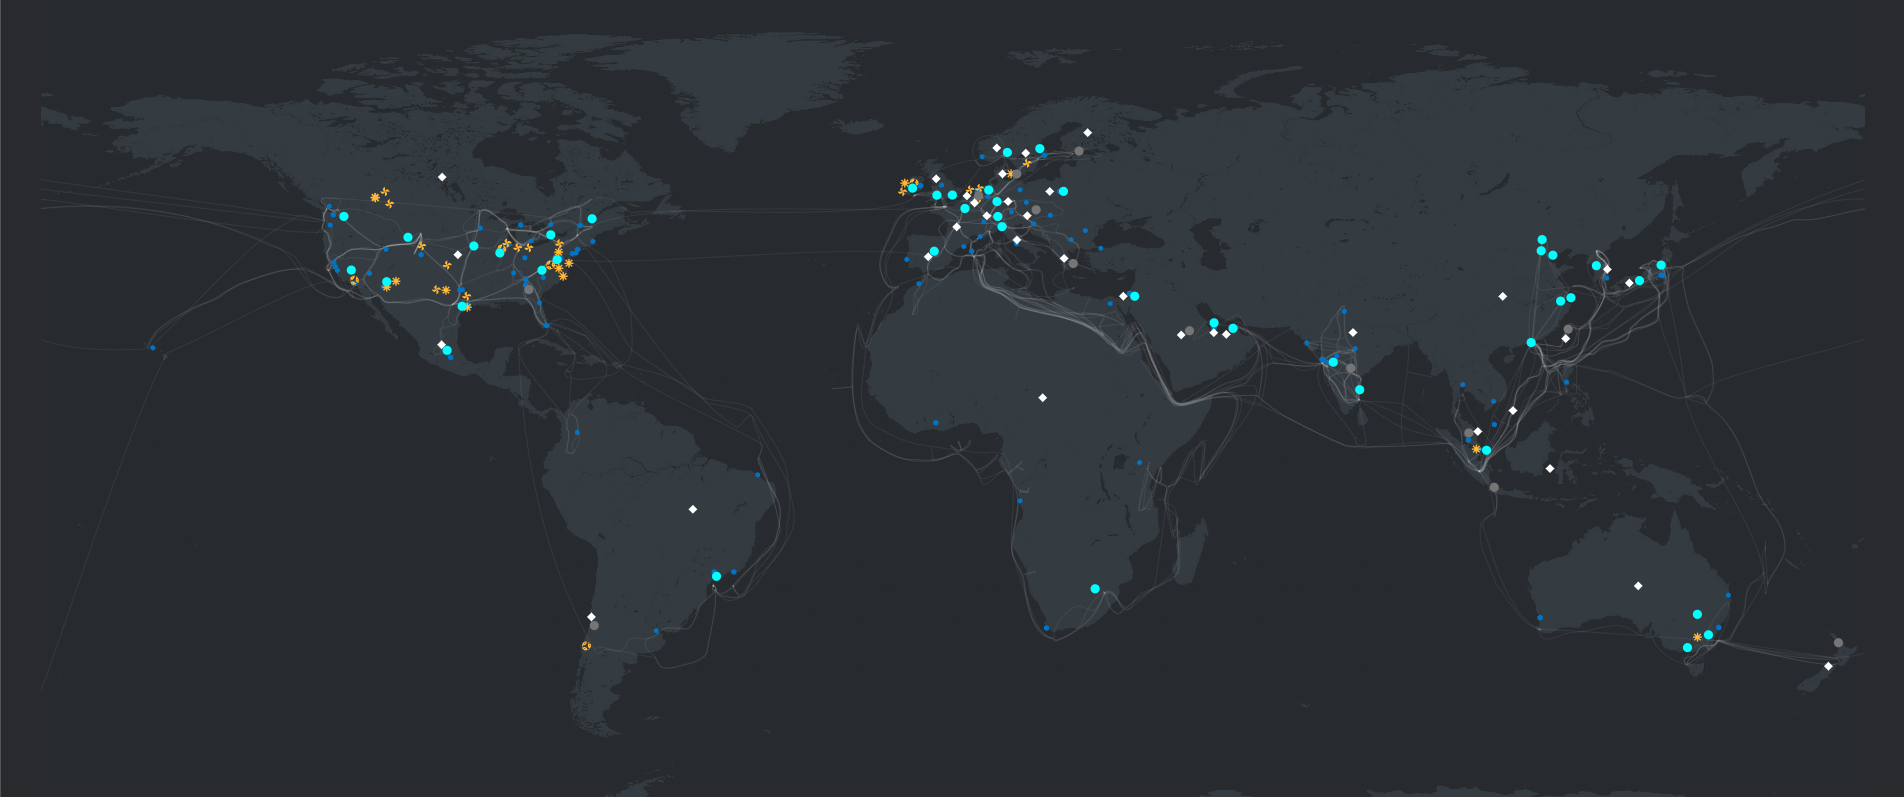
\includegraphics[width=\linewidth]{images/microsoft-datacenters.png}
	\label{fig:microsoft-datacenters}
  \source{\citeonline{azure_data_centers_locations}}
\end{figure}

\subsection{Computação em nuvem verde}

A computação verde é um paradigma que visa a criação de soluções tecnológicas ambientalmente sustentáveis e energeticamente eficientes. Esse conceito envolve o planejamento e o desenvolvimento de infraestruturas de computação e estratégias baseadas em princípios de gestão ambiental, otimização do consumo energético e práticas de reutilização. O objetivo central é promover a criação de produtos e serviços de tecnologia da informação (TI) que demandem menos energia e emitam menores quantidades de carbono. Nesse sentido, a computação verde busca reduzir o consumo de energia enquanto melhora a utilização da infraestrutura computacional, assegurando a expansão sustentável da computação em nuvem no longo prazo \cite{9793067}.

Em paralelo a esses esforços, tanto a academia quanto a indústria têm desenvolvido iniciativas para mitigar o impacto ambiental da computação em larga escala. Uma dessas iniciativas é o conceito de \textit{carbon-responsive computing} (CRC), que foca na priorização do uso de fontes de energia com menor intensidade de carbono, seja por meio de estratégias espaciais, temporais ou uma combinação de ambas. O CRC organiza-se em três estágios sequenciais, nos quais o progresso de cada fase depende da implementação adequada da anterior \cite{en14216917}.

O primeiro estágio, denominado \textit{carbon-aware computing}, compreende sistemas capazes de caracterizar e prever a intensidade de carbono, bem como medir o consumo energético associado. No segundo estágio, \textit{carbon-responsive computing}, as ações do sistema são orientadas pela intensidade de carbono em uso, ajustando o consumo energético conforme os níveis de emissões. Por fim, o terceiro estágio, \textit{carbon-resilient computing}, aborda a gestão e integração de elementos responsivos ao carbono, investigando as modificações necessárias nas infraestruturas de TI e de energia para reduzir a pegada de carbono e garantir maior resiliência ambiental \cite{en14216917}.

No contexto da infraestrutura geodistribuída da computação em nuvem, um dos principais mecanismos que permitem a implementação dessas estratégias ambientais é a migração ao vivo de máquinas virtuais, apresentada na Seção \ref{section:migracao-ao-vivo-maquinas-virtuais}. Como mencionado anteriormente, essa técnica possibilita a transferência de cargas de trabalho entre diferentes \textit{data centers} sem interrupções no serviço, promovendo o balanceamento de carga de maneira eficiente. Ao redirecionar o processamento para regiões onde a pegada de carbono é menor ou onde há disponibilidade de fontes de energia renováveis, a migração ao vivo contribui significativamente para a redução do impacto ambiental da computação em nuvem. Esse processo não só melhora a eficiência energética dos \textit{data centers}, como também apoia diretamente os objetivos de mitigação das emissões de carbono, e reforça o compromisso da computação verde com a sustentabilidade.

\section{Escalonamento}\label{section:escalonamento}

O escalonamento de tarefas é um desafio de otimização combinatória, no qual, dadas as características de um conjunto de recursos computacionais ($\alpha$) e de um conjunto de tarefas ($\beta$), o objetivo é encontrar uma alocação de recursos em tempo que minimize algum critério de otimização ($\gamma$). Essa formulação é frequentemente expressa pela notação \mbox{$\alpha$ $\vert$ $\beta$ $\vert$ $\gamma$}, introduzida por \citeonline{GRAHAM1979287}. Em ambientes de computação em nuvem, esses problemas de escalonamento ganham relevância à medida que a demanda por recursos computacionais cresce, exigindo alocações eficientes e dinâmicas que atendam a critérios como desempenho, economia de energia e sustentabilidade.

Um dos principais critérios de otimização nesse contexto é o \textit{makespan} ($C_{\max}$), que define o tempo em que a última tarefa de uma aplicação finaliza sua execução. Quando os recursos computacionais disponíveis são idênticos e conhecidos previamente, e o objetivo é minimizar o \textit{makespan} --- uma situação típica em problemas de escalonamento em \textit{clusters} --- o problema se torna fortemente NP-completo. Esse tipo de problema é denotado como $P\,\vert\,\vert\,C_{\max}$ \cite{GRAHAM1979287}.

No contexto desta dissertação, $\alpha$ representa os recursos computacionais disponíveis nos servidores dos \textit{data centers}, além de informações sobre a disponibilidade de fontes de energia com menor intensidade de carbono. Já $\beta$ descreve as exigências das VMs, como tempo de execução, prazos, memória e CPU. O critério $\gamma$ é a minimização do consumo de energia proveniente de fontes com alta intensidade de carbono, o que se alinha ao conceito de computação verde.

\chapter{Trabalhos correlatos}\label{chapter:trabalhos-correlatos}
Este capítulo apresenta a análise do estado da arte relacionada ao tema desta pesquisa. O objetivo da revisão é identificar, avaliar e sintetizar os estudos primários relevantes para responder às questões de pesquisa propostas. As questões tratadas na revisão são: (1) quais são as principais estratégias e algoritmos propostos na literatura para a migração de VMs com foco na redução de emissões de \ch{CO2} em \textit{data centers} geodistribuídos?; (2) quais são os impactos das diferentes técnicas de migração de VMs no \textit{downtime} das aplicações e no congestionamento de rede em ambientes geodistribuídos?; e (3) em que medida a utilização de fontes de energia de baixa intensidade de carbono influencia a eficácia das técnicas de migração para reduzir as emissões de \ch{CO2}?

O método seguido para realizar esta revisão, incluindo os detalhes do protocolo de revisão e sua condução, está descrito nos Apêndices \ref{chapter:protocolo-revisao-estado-da-arte} e \ref{chapter:resultados-conducao-revisao-estado-da-arte}. A revisão aborda a otimização da migração de VMs em DCs geodistribuídos, com o propósito de minimizar o impacto ambiental e melhorar a eficiência operacional. O foco é reduzir as emissões de \ch{CO2}, o \textit{downtime} das aplicações e o congestionamento de rede, além de otimizar o uso de fontes de energia de baixa intensidade de carbono.

\section{Gerenciamento de energia em \textit{data centers} em nuvem}

O consumo de energia em DCs em nuvem tem se tornado uma preocupação crescente devido ao alto custo operacional e ao impacto ambiental associado às emissões de carbono. Diversas pesquisas têm focado em estratégias para otimizar o uso de recursos, reduzir o consumo energético e manter os níveis de Qualidade de Serviço (QoS). Neste capítulo, discutimos abordagens relacionadas ao gerenciamento eficiente de energia em DCs, destacando técnicas de consolidação de VMs, algoritmos heurísticos e impactos na rede.

\subsection{Consolidação dinâmica de VMs e eficiência energética}

A consolidação dinâmica de VMs é uma estratégia amplamente utilizada para reduzir o consumo de energia em DCs. Ao migrar VMs de servidores subutilizados para outros servidores, é possível desligar máquinas físicas ociosas, economizando energia sem comprometer o desempenho das aplicações.

\citeonline{Guo20171335} propuseram métodos adaptativos para consolidação dinâmica de VMs, incluindo detecção de subutilização de \textit{hosts}, seleção de VMs para migração e algoritmos heurísticos baseados na análise de dados históricos. Os experimentos demonstraram redução significativa no consumo de energia e nas violações de SLA, evidenciando a eficácia da abordagem.

De forma similar, \citeonline{Ibrahim202081747} apresentaram o PAPSO, uma técnica baseada em \textit{Particle Swarm Optimization} (PSO) para consolidar VMs dinamicamente. O método busca minimizar o número de \textit{hosts} sobrecarregados e subutilizados, reduzindo a necessidade de migrações e, consequentemente, o consumo energético. Os resultados indicam melhorias em comparação com algoritmos tradicionais, como o \textit{Power-Aware Best Fit Decreasing}.

\citeonline{Al-Dulaimy2018185} abordaram a consolidação dinâmica de VMs, propondo uma abordagem distribuída que utiliza técnicas de limiar dinâmico para detectar \textit{hosts} subutilizados ou sobrecarregados. A estratégia de alocação de VMs é baseada no problema da mochila com múltiplas escolhas, otimizando o uso de recursos físicos e reduzindo o consumo de energia.

\citeonline{Supreeth20221892} apresentaram o VMS-EDMVM, uma abordagem de escalonamento dinâmico de VMs voltada para otimizar a eficiência energética. Utilizando o algoritmo Modified Weighted Linear Regression para detectar \textit{hosts} sobrecarregados e um modelo dinâmico para identificar \textit{hosts} subutilizados, o método reduziu o consumo de energia e as violações de SLA, demonstrando melhorias significativas em relação a abordagens anteriores.

A técnica híbrida KMGA, proposta por \citeonline{AskarizadeHaghighi20191367}, combina o algoritmo \textit{k-means} com um \textit{micro-genetic algorithm} para a consolidação dinâmica de VMs. Os experimentos demonstraram que o KMGA equilibra a redução de energia com o desempenho, minimizando o número de migrações em comparação com outras técnicas híbridas baseadas em PSO e GA.

Além disso, \citeonline{Gharehpasha20211293} propuseram um algoritmo que combina o \textit{Sine–Cosine Algorithm} (SCA) e o \textit{Salp Swarm Algorithm} (SSA) para alocação otimizada de VMs. O objetivo é minimizar o consumo de energia, reduzir o desperdício de recursos e diminuir as violações de SLA, evitando migrações excessivas. Os experimentos realizados com instâncias do Amazon EC2 demonstraram a superioridade do algoritmo em métricas como eficiência energética e utilização de recursos.

\citeonline{Liang2020329} apresentaram o algoritmo MALE (\textit{Memory-Aware Low-Energy}), que considera características de memória e CPU para gerenciar recursos de forma eficiente. O algoritmo prioriza tarefas com base em suas exigências de memória, ajustando a ordem de mapeamento e criação de VMs para reduzir simultaneamente o consumo de energia e os custos dos usuários. Os experimentos mostraram reduções significativas no tempo médio de execução de máquinas físicas e no consumo de energia.

Em ambientes de nuvem federada, \citeonline{Karthikeyan2023} propuseram um algoritmo de migração de VMs para reduzir consumo de energia e emissões de carbono, mantendo a disponibilidade de recursos e maximizando o lucro dos provedores. A abordagem utiliza níveis de sobreutilização e subutilização para realizar migrações dinâmicas, garantindo serviço contínuo mesmo em falhas de VMs. Resultados comparativos demonstraram que a técnica reduz emissões de carbono, consumo de energia e tempos de resposta, além de aumentar a precisão e o lucro em relação a métodos existentes.

\subsection{Algoritmos heurísticos e metaheurísticas para alocação de VMs}

A utilização de algoritmos heurísticos e metaheurísticas tem sido explorada para otimizar a alocação de VMs e reduzir o consumo de energia em DCs.

\citeonline{Chen2012177} apresentaram um algoritmo genético híbrido que considera recursos de CPU, rede e I/O de disco para escalonamento de recursos em nuvem. Embora tenha reduzido a ocupação de máquinas físicas em 30\% a 40\%, o elevado número de migrações de VMs foi identificado como um custo operacional relevante.

\citeonline{DineshReddy20191917} propuseram o MDPSO, uma versão modificada do PSO para alocação inicial de VMs e um algoritmo de seleção baseado em utilização de memória, largura de banda e tamanho das VMs. A abordagem busca otimizar o uso de recursos, reduzir máquinas físicas ativas e minimizar violações de SLA. Os experimentos demonstraram redução no consumo de energia em até 32\%.

O modelo ECO-VMAP, baseado em leilões combinatórios, foi apresentado por \citeonline{Gamsiz202118625}. O modelo permite que os usuários declarem complementaridades e substituibilidades entre VMs em seus lances e utiliza programação linear inteira para otimizar a alocação, minimizando o consumo de energia. Os resultados mostraram aumento nos lucros em 42\% em relação a sistemas FCFS e soluções próximas ao ótimo, dependendo da heurística utilizada.

\citeonline{Tseng2015556} propuseram os algoritmos heurísticos \textit{Tree} e \textit{Forest} para alocação de VMs orientada a serviços. Baseados em programação linear inteira, os algoritmos buscam reduzir custos de comunicação enquanto equilibram carga computacional, promovendo comunicações eficientes em ambientes de larga escala. Os resultados mostraram reduções significativas nos custos de comunicação externa e melhorias na eficiência energética.

\citeonline{Khodayarseresht2023} apresentaram o algoritmo heurístico ECAIVMP para alocação inicial de VMs com foco na eficiência energética e redução de emissões de carbono em DCs geodistribuídos. O algoritmo considera tanto o consumo de energia de TI quanto o de não-TI, otimizando a alocação sem comprometer a qualidade do serviço. Simulações mostraram que o ECAIVMP reduz o consumo de energia em 17\% e as emissões de carbono em 6\%, superando algoritmos concorrentes.

\citeonline{Huang2014902} propuseram dois algoritmos heurísticos dinâmicos de migração e consolidação de VMs para reduzir o consumo de energia e violações de SLA. Utilizando regressão local e programação dinâmica baseada no problema da mochila 0-1, os algoritmos reduziram significativamente o número de migrações, reinicializações de servidores e consumo de energia. Um dos algoritmos destacou-se por atingir o menor nível de violações de SLA.

\subsection{Impactos na nede e estratégias de migração de VMs}

O tráfego de rede e os custos de comunicação são fatores críticos ao considerar a migração de VMs e a alocação de recursos em DCs.

\citeonline{Shahzad2015140} propuseram um algoritmo de escalonamento que minimiza migrações de VMs, reduzindo congestionamento e latência na rede. Ao priorizar VMs com base em categorias, o algoritmo otimiza a utilização de recursos e reduz o overhead da comunicação, melhorando o equilíbrio de carga e minimizando os custos operacionais.

\citeonline{Teyeb2016798} abordaram o escalonamento de migração de VMs em DCs geodistribuídos, considerando o tempo de vida das VMs e o impacto no tráfego da rede backbone. Os resultados mostraram que o tempo de vida das VMs influencia diretamente o número de migrações e a estabilidade do sistema. A solução heurística proposta demonstrou eficácia na redução do tráfego de backbone, mantendo a estabilidade operacional.

\citeonline{Canali201743} propuseram um modelo que integra os impactos energéticos de computação e comunicação, incluindo o custo de migrações. O modelo reduz o consumo de energia ao considerar tanto a transferência de dados quanto a sobrecarga computacional das migrações, alcançando reduções de até 60\% no consumo energético em comparação com abordagens que desconsideram o impacto energético da comunicação.

\citeonline{Ferdaus201765} introduziram o algoritmo NDAP para alocação simultânea de VMs e blocos de dados, visando reduzir custos de comunicação e tráfego de rede. O NDAP mostrou-se eficaz na redução do custo médio de rede em até 67\% e do uso de switches centrais em até 84\%, apesar de sua complexidade quadrática.

\citeonline{Addya20192877} propuseram um \textit{framework} para migração ao vivo de VMs, analisando estratégias de migração serial, paralela e serial aprimorada. Os resultados mostraram que a migração paralela minimiza o \textit{downtime}, enquanto a migração serial aprimorada reduz o tempo total de migração e é mais eficiente em termos de energia. A abordagem oferece insights sobre custos e eficiência em cenários de federação de nuvens.

\citeonline{Satpathy2021} apresentaram uma estratégia de migração serial modificada para múltiplas VMs baseada na técnica de pré-cópia. A abordagem equilibra os estágios de pré-cópia, otimizando o desempenho em aplicações de \textit{big data} com cargas de trabalho variáveis e requisitos de baixa latência. Os resultados mostram que, para aplicações com altas taxas de escrita, a técnica supera significativamente as estratégias paralelas em termos de \textit{downtime}.

\citeonline{Ye2011267} avaliaram a eficiência da migração ao vivo de múltiplas VMs considerando diferentes métodos de reserva de recursos e estratégias avançadas, como migração paralela e consciente de carga. Os resultados mostraram que a reserva de recursos é essencial para evitar falhas e melhorar a eficiência das migrações. A estratégia de migração consciente de carga melhora o desempenho das cargas transferidas.

\citeonline{Vakilinia2018} propuseram uma otimização conjunta do consumo de energia de servidores, comunicação de rede e custos de migração, utilizando um programa quadrático inteiro. A abordagem aplica a técnica de geração de colunas para sistemas maiores, reduzindo significativamente o consumo de energia em comparação com algoritmos heurísticos.

\subsection{Considerações sobre qualidade de serviço}

Manter a qualidade de serviço é essencial ao implementar estratégias de economia de energia. É necessário equilibrar a redução do consumo energético com o cumprimento dos Acordos de Nível de Serviço (SLAs).

\citeonline{Guérout2014225} avaliaram algoritmos de escalonamento utilizando múltiplos parâmetros de QoS, como consumo de energia, tempo de resposta, robustez e dinamismo. Os resultados destacam que algoritmos genéticos podem equilibrar múltiplos objetivos, permitindo otimizações eficientes entre consumo de energia e tempo de resposta. A inclusão de mais métricas na análise revelou diferenças significativas nos resultados, reforçando a importância de uma abordagem multiobjetivo.

\citeonline{Mandal20207374} e \citeonline{Mandal2023651} propuseram políticas de seleção de VMs conscientes de energia para migração, visando reduzir o consumo energético e as emissões de carbono, minimizando violações de SLA. Os resultados mostram que as políticas otimizam a seleção de VMs para migração, equilibrando eficiência energética e manutenção de SLAs.

\citeonline{Supreeth20221892} apresentaram o VMS-EDMVM, já discutido anteriormente, que reduz o consumo de energia e as violações de SLA através de técnicas de detecção de \textit{hosts} sobrecarregados e subutilizados e uma estratégia de escalonamento em duas fases.

\citeonline{Al-Dulaimy2018185}, já mencionado, também destacam a importância de técnicas que consideram a QoS ao propor uma abordagem distribuída para consolidação dinâmica de VMs, utilizando técnicas de limiar dinâmico para superar as limitações de limiares estáticos em cenários de carga imprevisível.

\subsection{Computação em nuvem verde e sustentabilidade ambiental}

A preocupação com a sustentabilidade ambiental tem motivado pesquisas focadas na redução das emissões de carbono em DCs.

\citeonline{Wadhwa20142297} propuseram a técnica CEPM (\textit{Carbon Efficient Placement and Migration}) para reduzir emissões de carbono e consumo de energia. A abordagem utiliza a taxa de pegada de carbono dos DCs geodistribuídos e técnicas de alocação e migração de VMs para otimizar o escalonamento de forma ambientalmente eficiente.

\citeonline{Khosravi2017} desenvolveram algoritmos para migração de VMs entre DCs com o objetivo de aproveitar fontes de energia renovável e reduzir custos. Foram desenvolvidos um algoritmo \textit{offline} com conhecimento total do futuro e dois algoritmos \textit{online}: um determinístico sem previsão e outro \textit{future-aware} com janela de previsão limitada. Os resultados mostram que algoritmos com previsão de disponibilidade de energia renovável podem se aproximar da eficiência de algoritmos com conhecimento total do futuro.

\citeonline{Khodayarseresht2023} apresentaram o algoritmo ECAIVMP, já discutido, focado na alocação inicial de VMs com eficiência energética e redução de emissões de carbono em DCs geodistribuídos. O algoritmo considera o consumo de energia de TI e não-TI, otimizando a alocação sem comprometer a qualidade do serviço.

\citeonline{Xu201987} introduziram o VMSAGE, um algoritmo de escalonamento de VMs inspirado no modelo de gravitação física, que otimiza a eficiência energética ao considerar fatores como repulsão térmica e gravitação lógica entre VMs, \textit{hosts} e \textit{racks}. Os resultados experimentais mostram que o VMSAGE reduz o consumo de energia em 20\% em comparação ao DVFS e em 10\% em relação ao BFH.

\citeonline{Liang2020329} apresentaram o algoritmo MALE, que considera características de memória e CPU para reduzir o consumo de energia e os custos dos usuários, contribuindo para práticas de computação em nuvem verde. O algoritmo prioriza tarefas baseadas em suas exigências de memória, ajustando a ordem de mapeamento de tarefas e a criação de VMs.

\citeonline{More201773} revisaram técnicas e algoritmos relacionados à consolidação de VMs para reduzir o consumo de energia, destacando a importância de parâmetros como servidores, CPUs e dispositivos de rede na eficiência energética. O trabalho propõe uma equação inicial para calcular o consumo energético e sugere explorar métricas como flops/watt para otimizar o uso de recursos e minimizar emissões de \ch{CO2}.

\subsection{Aplicações HPC em ambientes de nuvem}

O suporte a cargas de trabalho de \textit{High-Performance Computing} (HPC) em ambientes de nuvem traz desafios adicionais relacionados à eficiência energética e ao gerenciamento de recursos.

\citeonline{Rodero2012447} propuseram soluções reativas e proativas para gerenciar anomalias térmicas e otimizar a alocação de VMs para cargas HPC. A solução reativa combina migração de VMs, DVFS e \textit{CPU pinning}, enquanto a proativa utiliza perfis de aplicação para maximizar eficiência energética e QoS. Os experimentos demonstraram reduções de 12\% no consumo de energia e 18\% no tempo de execução das aplicações.

\citeonline{Ye2011267}, já mencionados, avaliaram a eficiência da migração ao vivo de múltiplas VMs, o que é relevante para cargas HPC que exigem alta disponibilidade e desempenho. Os resultados mostram que a migração ao vivo gera sobrecargas de desempenho que variam conforme o tamanho da memória, recursos de CPU e tipo de carga de trabalho.

\subsection{Heurísticas e técnicas de migração avançadas}

Diversas pesquisas focaram em aprimorar as técnicas de migração de VMs para melhorar a eficiência energética e o desempenho.

\citeonline{Mishra201234} exploraram o papel essencial da migração ao vivo de VMs no gerenciamento dinâmico de recursos, destacando sua importância para consolidação, balanceamento de carga e mitigação de hotspots. O estudo categoriza as heurísticas de migração com base nos componentes principais do processo: quando migrar, qual VM migrar e para onde migrar.

\citeonline{Sun2018279} apresentaram o algoritmo VDC-M para migração de múltiplas VMs correlacionadas, otimizando o desempenho da migração em termos de custo de remapeamento e \textit{downtime}. Os resultados experimentais mostram que o VDC-M supera o algoritmo benchmark VDC-SM em eficiência de remapeamento e redução de \textit{downtime}.

\citeonline{Huang2014902} propuseram algoritmos heurísticos para migração e consolidação de VMs, já discutidos, que reduziram significativamente o número de migrações e o consumo de energia, além de atingir menor nível de violações de SLA.

\citeonline{Tseng2015556} apresentaram os algoritmos \textit{Tree} e \textit{Forest}, já mencionados, que buscam reduzir custos de comunicação e equilibrar a carga computacional. O algoritmo \textit{Tree} reduziu os custos de comunicação externa em 92\%, enquanto o \textit{Forest} diminuiu esses custos em 22\%.

\citeonline{Addya20192877} propuseram um \textit{framework} para migração ao vivo de VMs, analisando diferentes estratégias e oferecendo insights sobre custos e eficiência em cenários de federação de nuvens. A migração serial aprimorada mostrou-se eficiente em termos de energia.

\subsection{Redução de consumo de energia em \textit{data centers} federados}

Em ambientes de nuvem federada, estratégias específicas são necessárias para otimizar o consumo de energia.

\citeonline{Karthikeyan2023}, já discutido, propuseram um algoritmo de migração de VMs que reduz o consumo de energia e as emissões de carbono, mantendo a disponibilidade de recursos e maximizando o lucro dos provedores. A abordagem utiliza categorização de DCs baseada em MIPS e custos antes da alocação de tarefas, otimizando o uso de recursos.

\citeonline{Satpathy2021}, já mencionado, apresentaram uma estratégia de migração eficiente para múltiplas VMs, relevante para ambientes federados que exigem baixa latência e migrações eficientes. A solução é eficaz para cenários em que baixa latência e migrações eficientes são cruciais.

\section{Considerações Finais}

A otimização do consumo de energia em DCs em nuvem é um desafio multidimensional que envolve balancear eficiência energética, qualidade de serviço e desempenho operacional. As pesquisas discutidas neste capítulo abordam diferentes aspectos desse problema, desde a consolidação dinâmica de VMs e o uso de algoritmos heurísticos até considerações sobre impactos na rede e sustentabilidade ambiental.

Estratégias que combinam técnicas de migração eficiente, alocação inteligente de recursos e consideração de múltiplos parâmetros de desempenho mostram-se promissoras para alcançar DCs mais sustentáveis e eficientes. No entanto, é necessário continuar explorando novas abordagens que integrem avanços tecnológicos, como fontes de energia renovável e técnicas de aprendizado de máquina, para aprimorar ainda mais a gestão de recursos em ambientes de computação em nuvem.

% ----------------------------------------------------------
% ELEMENTOS PÓS-TEXTUAIS
% ----------------------------------------------------------
\postextual
% ----------------------------------------------------------

% ----------------------------------------------------------
% Referências bibliográficas
% ----------------------------------------------------------
\bibliography{referencias}

% ----------------------------------------------------------
% Glossário
% ----------------------------------------------------------
%
% Consulte o manual da classe abntex2 para orientações sobre o glossário.
%
%\glossary

% ----------------------------------------------------------
% Apêndices
% ----------------------------------------------------------

% ---
% Inicia os apêndices
% ---
\begin{apendicesenv}

% Imprime uma página indicando o início dos apêndices
%\partapendices

%-------------------------------------------------------------------------
% Comentário adicional do PPgSI - Informações sobre ``apêndice''
%
% Para todos os captions/(títulos) (de seções, subseções, tabelas, 
% ilustrações, etc.):
%     - em maiúscula apenas a primeira letra da sentença (do título), 
%       exceto nomes próprios, geográficos, institucionais ou Programas ou
%       Projetos ou siglas, os quais podem ter letras em maiúscula também.
%
% Todas  as tabelas, ilustrações (figuras, quadros, gráficos etc. ), 
% anexos, apêndices devem obrigatoriamente ser citados no texto.
%      - a citação deve vir sempre antes da primeira vez em que a tabela, 
%        ilustração etc., aparecer pela primeira vez.
%
%-------------------------------------------------------------------------
\chapter{Protocolo da revisão do estado da arte}\label{chapter:protocolo-revisao-estado-da-arte}

\section{Tema da revisão}\label{section:tema-da-revisao}

A revisão aborda a otimização da migração de VMs em \textit{data centers} geodistribuídos, com o propósito de minimizar o impacto ambiental e melhorar a eficiência operacional. O foco é reduzir as emissões de \ch{CO2}, o \textit{downtime} das aplicações e o congestionamento de rede, além de otimizar o uso de fontes de energia de baixa intensidade de carbono. A revisão busca também avaliar como a combinação de diferentes algoritmos e técnicas de migração pode contribuir para alcançar uma operação mais sustentável e eficiente em cenários com energia renovável parcial ou total.

\section{Tipo de revisão}\label{section:tipo-de-revisao}

Esta revisão será conduzida no formato de revisão de escopo. Uma revisão de escopo é um tipo de revisão que busca mapear a literatura científica disponível sobre um tema específico, identificando as principais abordagens, lacunas e tendências na área de pesquisa. É mais abrangente que a abordagem sistemática, com o objetivo de fornecer uma visão geral do campo de estudo e descrever a amplitude dos tópicos abordados.

A escolha pela revisão de escopo se justifica pela necessidade de explorar diversas estratégias e técnicas de migração de VMs em \textit{data centers} geodistribuídos, considerando os muitos aspectos que impactam a eficiência energética, sustentabilidade e desempenho operacional. Dado o caráter multidisciplinar e a constante evolução tecnológica no tema, é essencial mapear o estado atual da literatura para identificar lacunas no conhecimento e oportunidades para futuros desenvolvimentos. Dessa forma, a revisão de escopo servirá como uma base estruturada para direcionar pesquisas futuras e propor novas abordagens na minimização de emissões de carbono e na otimização da migração de VMs em ambientes \textit{cloud} sustentáveis.

\section{Questões de pesquisa}\label{section:questoes-de-pesquisa}
Considerando a necessidade de uma revisão de escopo, um conjunto de questões de pesquisa foi definido para este trabalho. Essas questões estão voltadas para explorar as práticas e técnicas de migração de VMs em \textit{data centers} geodistribuídos, especialmente no contexto da minimização das emissões de \ch{CO2} e da otimização do uso de fontes de energia de baixa intensidade de carbono. O principal interesse deste estudo é identificar e avaliar os trabalhos que abordam essas técnicas e estratégias, visando uma compreensão abrangente da área de pesquisa. Através dessas questões, busca-se não apenas mapear as abordagens existentes, mas também destacar as lacunas na literatura que podem ser exploradas em investigações futuras.

\textbf{Q1}: Quais são as principais estratégias e algoritmos propostos na literatura para a migração de VMs com foco na redução de emissões de \ch{CO2} em \textit{data centers} geodistribuídos?

A finalidade desta questão é identificar as principais estratégias e algoritmos que têm sido abordados na literatura sobre migração de VMs, especialmente aqueles voltados para a minimização das emissões de \ch{CO2} em \textit{data centers} geodistribuídos. Para esta questão, foram consideradas as categorias de migração, incluindo migração baseada em \textit{threshold} e otimização multiobjetivo.

\textbf{Q2}: Quais são os impactos das diferentes técnicas de migração de VMs no \textit{downtime} das aplicações e no congestionamento de rede em ambientes geodistribuídos?

A finalidade desta questão é avaliar os impactos que as diversas técnicas de migração de VMs têm no \textit{downtime} das aplicações e no congestionamento da rede, considerando o contexto de \textit{data centers} geodistribuídos. Para esta análise, serão utilizadas métricas de desempenho relatadas na literatura, como tempo médio de migração e latência de rede, permitindo uma comparação sistemática. A escolha dessas métricas se justifica pela relevância que têm na qualidade do serviço prestado, além de sua aplicabilidade em diferentes cenários operacionais.

\textbf{Q3}: Em que medida a utilização de fontes de energia de baixa intensidade de carbono influencia a eficácia das técnicas de migração para reduzir as emissões de \ch{CO2}?

A finalidade desta questão é investigar como a utilização de fontes de energia de baixa intensidade de carbono influencia a eficácia das técnicas de migração de VMs na redução das emissões de \ch{CO2}. Para abordar esta questão, serão analisados estudos que consideram diferentes tipos de fontes energéticas e seus impactos nas técnicas de migração. A correlação entre a intensidade de carbono das fontes energéticas e a eficiência das técnicas será avaliada, destacando os cenários em que essas técnicas se mostram mais eficazes. Essa abordagem é relevante, pois permite uma compreensão mais clara de como a escolha da fonte de energia pode otimizar a operação dos \textit{data centers} em termos de sustentabilidade.

\section{Bases de dados usadas}\label{section:bases-de-dados-usadas}

A única base de dados utilizada para a realização do protocolo de revisão foi o Scopus, por ser bem estabelecida como a maior base de dados de literatura revisada por pares. Devido ao grande número de bases de dados indexadas pelo Scopus, esta revisão de escopo também abrangeu universidades editoras e outras associações científicas. Pesquisas diretas no IEEE, ACM ou bibliotecas Springer, por exemplo, seriam redundantes e, portanto, desnecessárias.

\section{String de busca}\label{section:string-de-busca}

Foi criada uma \textit{string} de busca contendo palavras-chave relacionadas à migração ao vivo de máquinas virtuais em \textit{datacenters} geodistribuidos com foco em computação sustentável. A sequência de busca compreende disjunções de termos genéricos com agrupamentos incluídos na literatura especializada. Além disso, a sequência de busca possui uma segunda parte destinada a filtrar apenas por artigos especificamente que mencionem máquinas virtuais e não sejam de computação de borda ou em névoa. Uma representação para a \textit{string} de busca é fornecida na Tabela \ref{tab:StringDeBusca}.

\begin{table}[htbp]
	\centering
	\caption{\textit{String} de busca}
		\begin{tabular}{p{6in} } \hline
			("virtual machine" OR vm) AND "live migration" AND (("energy*" OR "power*") AND ("saving" OR "optimization" OR "aware" OR "efficiency")) AND ("cloud" OR "data center") AND ("sustainable computing" OR "green computing") AND NOT ("fog computing" OR "edge computing") AND NOT TITLE(consolidation)
		\end{tabular}
	\label{tab:StringDeBusca}
\end{table}

\section{Estratégia de seleção de estudos primários}\label{section:estrategia-de-selecao-de-estudos-primarios}

Como resultados falso-positivos podem ser retornados devido ao amplo espectro da \textit{string} de busca, esses resultados precisam ser verificados.

\begin{table}[htbp]
	\centering
	\caption{Critério de Inclusão (CI)}
		\begin{tabular}{p{1in} p{5in} } \hline

		CI-1	& O principal objetivo da pesquisa ou um dos objetivos específicos do estudo é a otimização de uma ou mais métricas de gerenciamento de máquinas virtuais em \textit{datacenters} geodistribuidos \\
		CI-2	& O estudo aborda a aplicação de técnicas para otimização de uma ou mais métricas de gerenciamento de máquinas virtuais em \textit{datacenters} geodistribuidos e discute os resultados de sua aplicação \\ \hline

		\end{tabular}
	\label{tab:TabelaCriteriosInclusao}
\end{table}

\begin{table}[htbp]
	\centering
	\caption{Critério de Exclusão (CE)}
		\begin{tabular}{p{1in} p{5in} } \hline

		CE-1	& O estudo não está completamente em inglês \\
		CE-2	& O estudo não está relacionado a ciência da computação, sistemas de informação, engenharia ou campo fortemente relacionado \\
		CE-3	& O estudo não é primário \\ \hline

		\end{tabular}
	\label{tab:TabelaCriteriosExclusao}
\end{table}

As Tabelas \ref{tab:TabelaCriteriosInclusao} e \ref{tab:TabelaCriteriosExclusao} apresentam, respectivamente, os Critérios de Inclusão (CI) e os Critérios de Exclusão (CE) definido para esta verificação. Para que um estudo seja selecionado como estudo primário, deve atender a todos os critérios de inclusão e a nenhum critério de exclusão.

\section{Estratégia para extração de dados e para síntese de resultados}\label{section:estrategia-para-extracao-de-dados-e-para-sintese-de-resultados}

Os artigos selecionados para inclusão foram lidos em completo para extração de resultados. A leitura foi orientada pelas questões de pesquisa (\ref{section:questoes-de-pesquisa}). Durante a leitura, foram copiados trechos de artigos que auxiliavam a responder às questões de pesquisa para controlar planilhas. O conjunto de trechos referentes a cada questão de pesquisa respaldada tanto a elaboração das respostas correspondentes como a reunião dos pontos fortes e pontos fracos do estado da arte em gerenciamento de máquinas virtuais em \textit{datacenters} geodistribuidos com foco em computação sustentável.

\chapter{Resultados da condução da revisão estado da arte}\label{chapter:resultados-conducao-revisao-estado-da-arte}

\section{Relato da condução}\label{section:relato-da-conducao}

Para encontrar estudos candidatos para estudos primários, a \textit{string} de busca foi aplicada sobre os campos título, resumo e palavras-chave, no mecanismo de busca Scopus. A \textit{string} base (\ref{tab:StringDeBusca}) foi ampliada com filtros adicionais que permitiram a aplicação automática da exclusão critérios CE-1 e CE-2 para restringir o idioma de escrita (somente em inglês), bem como os campos em que os trabalhos poderiam estar associados (ciências da computação e engenharia). Esta fase foi realizada em outubro de 2024 e resultou em 408 estudos candidatos.

Dos 408 artigos, 27 foram excluídos pelo critério CE-3 e outros 342 não atenderam a nenhum critério de inclusão; desta forma, restaram 38 artigos.

\begin{figure}[htbp]
	\centering
	\caption{Processo de seleção dos artigos primários}
		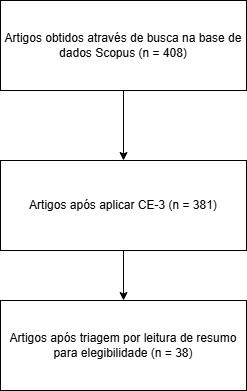
\includegraphics[width=.3\linewidth]{images/seleção-dos-artigos-primários.png}
	\label{fig:seleção-dos-artigos-primários}
  \source{Autor (2024)}
\end{figure}

\section{Tabela com os artigos primários selecionados}\label{section:tabela-com-os-artigos-primarios-selecionados}

A Tabela \ref{tab:EstudosPrimariosSelecionados} contempla os artigos primários selecionados.

\begin{longtable}{|p{3in}|p{2in}|p{1in}|}
	\caption{Estudos primários selecionados}
	\label{tab:EstudosPrimariosSelecionados} \\
	\hline
	\textbf{Título} & \textbf{Autores (Ano de publicação)} \\
	\hline
	Quality of service modeling for green scheduling in Clouds & \citeonline{Guérout2014225} \\
	\hline 
	Evaluating impact of live migration on data center energy saving & \citeonline{Akiyama2015759} \\
	\hline 
	A cloud computing resource scheduling policy based on genetic algorithm with multiple fitness & \citeonline{Chen2012177} \\
	\hline 
	Reduce VM migration in bandwidth oversubscribed cloud data centres & \citeonline{Shahzad2015140} \\
	\hline 
	Traffic-aware virtual machine migration scheduling problem in geographically distributed data centers & \citeonline{Teyeb2016798} \\
	\hline
	A computation- Network-Aware energy optimization model for virtual machines allocation & \citeonline{Canali201743} \\
	\hline
	Heuristic algorithms for energy and performance dynamic optimization in cloud computing & \citeonline{Guo20171335} \\
	\hline
	Carbon efficient VM placement and migration technique for green federated cloud datacenters & \citeonline{Wadhwa20142297} \\
	\hline
	Dynamic Virtual Machine migration algorithms using enhanced energy consumption model for green cloud data centers & \citeonline{Huang2014902} \\
	\hline
	Dynamic resource management using virtual machine migrations & \citeonline{Mishra201234} \\
	\hline
	Energy-Efficient Thermal-Aware Autonomic Management of Virtualized HPC Cloud Infrastructure & \citeonline{Rodero2012447} \\
	\hline
	Live migration of multiple virtual machines with resource reservation in cloud computing environments & \citeonline{Ye2011267} \\
	\hline
	Hybrid soft computing approach for energy efficiency in cloud computing & \citeonline{Jasuja2016} \\
	\hline
	Service-Oriented Virtual Machine Placement Optimization for Green Data Center & \citeonline{Tseng2015556} \\
	\hline
	Online virtual machine migration for renewable energy usage maximization in geographically distributed cloud data centers & \citeonline{Khosravi2017} \\
	\hline
	Type-aware virtual machine management for energy efficient cloud data centers & \citeonline{Al-Dulaimy2018185} \\
	\hline
	Live Migration for Multiple Correlated Virtual Machines in Cloud-Based Data Centers & \citeonline{Sun2018279} \\
	\hline
	An algorithm for network and data-aware placement of multi-tier applications in cloud data centers & \citeonline{Ferdaus201765} \\
	\hline
	Energy efficient temporal load aware resource allocation in cloud computing datacenters & \citeonline{Vakilinia2018} \\
	\hline
	Challenges in green computing for energy saving techniques & \citeonline{More201773} \\
	\hline
	PAPSO: A power-aware VM placement technique based on particle swarm optimization & \citeonline{Ibrahim202081747} \\
	\hline
	Energy aware virtual machine scheduling in data centers & \citeonline{Qiu2019} \\
	\hline
	A Strategy for Live Migration of Virtual Machines in a Cloud Federation & \citeonline{Addya20192877} \\
	\hline
	Memory-aware resource management algorithm for low-energy cloud data centers & \citeonline{Liang2020329} \\
	\hline
	VMSAGE: A virtual machine scheduling algorithm based on the gravitational effect for green Cloud computing & \citeonline{Xu201987} \\
	\hline
	Energy-aware virtual machine allocation and selection in cloud data centers & \citeonline{DineshReddy20191917} \\
	\hline
	An Energy-Aware Combinatorial Virtual Machine Allocation and Placement Model for Green Cloud Computing & \citeonline{Gamsiz202118625} \\
	\hline
	An approach toward design and development of an energy-aware VM selection policy with improved SLA violation in the domain of green cloud computing & \citeonline{Mandal20207374} \\
	\hline
	An Energy-Efficient Dynamic Resource Management Approach Based on Clustering and Meta-Heuristic Algorithms in Cloud Computing IaaS Platforms: Energy Efficient Dynamic Cloud Resource Management & \citeonline{AskarizadeHaghighi20191367} \\
	\hline
	Energy and carbon-aware initial VM placement in geographically distributed cloud data centers & \citeonline{Khodayarseresht2023} \\
	\hline
	VM Scheduling for Efficient Dynamically Migrated Virtual Machines (VMS-EDMVM) in Cloud Computing Environment & \citeonline{Supreeth20221892} \\
	\hline
	A Service Sustainable Live Migration Strategy for Multiple Virtual Machines in Cloud Data Centers & \citeonline{Satpathy2021} \\
	\hline
	Preserving Resource Handiness and Exigency-Based Migration Algorithm (PRH-EM) for Energy Efficient Federated Cloud Management Systems & \citeonline{Karthikeyan2023} \\
	\hline
	Power efficient virtual machine placement in cloud data centers with a discrete and chaotic hybrid optimization algorithm & \citeonline{Gharehpasha20211293} \\
	\hline
	MECpVmS: an SLA aware energy-efficient virtual machine selection policy for green cloud computing & \citeonline{Mandal2023651} \\
	\hline
\end{longtable}

\section{Análise descritiva}\label{section:analise-descritiva}

Através da Figura \ref{fig:artigos-por-ano} é possivel perceber que o interesse científico pelo assunto, desde que surgiu, é constante.
\begin{figure}[htbp]
	\centering
	\caption{Distribuição dos artigos selecionados no tempo}
		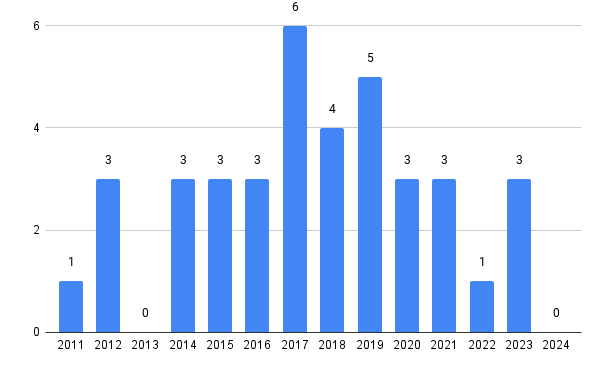
\includegraphics[width=\linewidth]{images/artigos-por-ano.png}
	\label{fig:artigos-por-ano}
  \source{Autor (2024)}
\end{figure}

A maior parte dos artigos selecionados foram publicados em periódicos, conforme mostra a Figura \ref{fig:local-de-publicação-do-artigo}.
\begin{figure}[htbp]
	\centering
	\caption{Local de publicação dos artigos selecionados}
		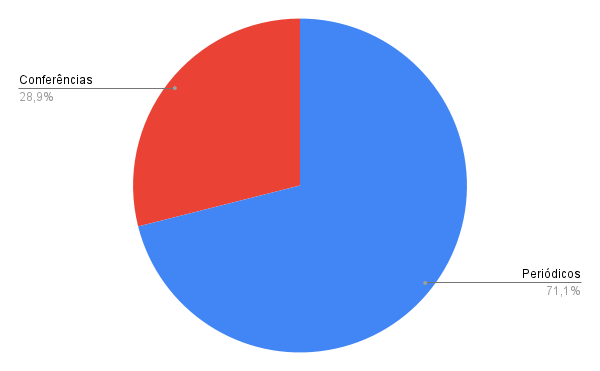
\includegraphics[width=\linewidth]{images/local-de-publicação-do-artigo.png}
	\label{fig:local-de-publicação-do-artigo}
  \source{Autor (2024)}
\end{figure}

\end{apendicesenv}
% ---


% ----------------------------------------------------------
% Anexos
% ----------------------------------------------------------

% ---
% Inicia os anexos
% ---
\begin{anexosenv}

% Imprime uma página indicando o início dos anexos
%\partanexos

\end{anexosenv}

%---------------------------------------------------------------------
% INDICE REMISSIVO
%---------------------------------------------------------------------
%%%%%MF\phantompart
%%%%%MF\printindex
%---------------------------------------------------------------------

\end{document}
